% !TeX program = xelatex

\documentclass[letterpaper,10pt,conference]{IEEEtran}

\usepackage{amsmath,amssymb}
\usepackage{graphicx}
\usepackage{booktabs}
\usepackage{array}
\usepackage{multirow}
\usepackage{tabularx}
\usepackage{listings}
\usepackage{cite}
\usepackage[hyphens]{url}
\usepackage[hidelinks]{hyperref}
\usepackage[table]{xcolor}
\usepackage{xeCJKfntef}

% Temporary review-only yellow highlighting. This implementation supports
% line breaks in long English spans and avoids soul/hl reconstruction issues.
\newcommand{\REV}[1]{%
  \CJKunderline[
    thickness=1.15em,
    depth=-0.15em,
    format=\color{yellow}
  ]{#1}%
}

\lstset{
  basicstyle=\ttfamily\scriptsize,
  breaklines=true,
  breakatwhitespace=false,
  columns=fullflexible,
  keepspaces=true,
  showstringspaces=false
}

\title{TEF-RAG: Temporal Evidence Flow Retrieval-Augmented Generation}
\author{Juxian Yin}

\newcommand{\ind}{\mathbb{I}}
\newcommand{\Rels}{\mathcal{R}}
\newcommand{\Evidence}{\mathcal{K}}
\newcommand{\Candidates}{\mathcal{C}}
\newcommand{\FlowGraph}{\mathcal{G}}
\newcommand{\SetBank}{\mathcal{B}}
\newcommand{\Selected}{\mathcal{S}}
\newcommand{\placeholderfigure}[1]{%
  \fbox{\parbox{0.94\linewidth}{\vspace{0.8in}\centering\textit{#1}\par\vspace{0.8in}}}%
}

\begin{document}

\maketitle

% =========================================================
% Abstract
% =========================================================
\begin{abstract}
Retrieval-augmented generation for embodied operation and maintenance (O\&M) in energy-storage 
stations must do more than retrieve records that are semantically relevant to a query. 
It must also ensure that the evidence was actually available at the query time and 
that the retrieved records can jointly support a complete process from state observation 
and diagnosis to action and verification. We propose TEF-RAG (Temporal Evidence 
Flow Retrieval-Augmented Generation), which formulates retrieval in dynamic O\&M 
environments as query-conditioned temporal evidence-flow selection. TEF-RAG first 
applies deterministic constraints on asset identity, event time, availability time, 
and procedure applicability. A learned pair proposal module then selects evidence 
pairs worth semantic relation reasoning, and a directed graph is constructed with 
relations such as support, update, qualification, supersession, and verification. 
Finally, a nonlinear RankNet learns set-level relative utility over candidate 
evidence sets and selects an evidence flow of at most five records with complementary 
roles and coherent relations. We construct a public-source-grounded benchmark with 
dual timestamps, supersession, cross-source complementary evidence, and persistent 
uncertainty, and compare different retrieval contexts under a shared downstream generator. 
\REV{On the test split, TEF-RAG records the highest Recall@5, Complete@5, and FlowComplete@5 
among the six compared methods. Under the 
shared generator, TEF-RAG records the highest Field Macro F1, Action F1, Citation F1, and 
Evidence Support Recall.} The results support evaluating retrieval at the evidence-set 
level when temporal visibility and cross-record relations are part of the task definition.
\end{abstract}

% =========================================================
\section{Introduction}
\label{sec:introduction}
% =========================================================

Knowledge for operation and maintenance (O\&M) in energy-storage stations is inherently dynamic and process-oriented. Handling a single anomaly often requires jointly consulting equipment states, alarms and inspection records, historical work orders, operating procedures, and post-action verification results. Unlike static knowledge question answering, the system must answer two stricter questions in addition to identifying which evidence is relevant to the query: whether that evidence was already available at the query time, and whether the evidence can jointly form a complete process that supports the current decision.

Retrieval-augmented generation (RAG) combines language models with external retrieval for knowledge-intensive generation~\cite{lewis2020rag}. On the retrieval side, BM25 remains a strong lexical baseline, while neural retrievers such as DPR and ColBERT improve semantic matching through dense representations or late interaction~\cite{karpukhin2020dpr,khattab2020colbert}; BEIR further shows that retrieval paradigms differ substantially in cross-domain generalization~\cite{thakur2021beir}. On the generation side, FiD demonstrates that a generator can effectively aggregate multiple retrieved passages~\cite{izacard2021fid}, while Self-RAG further studies joint control over retrieval, generation, and self-reflection~\cite{asai2024selfrag}.

However, conventional RAG typically treats candidate documents as independent relevance units. This assumption is insufficient for continuously updated O\&M records. First, O\&M evidence has dual temporal attributes: the event time and the time at which the record becomes available to the system need not coincide, and late-arriving records must not be used retrospectively by an earlier query. Second, maintenance decisions usually depend on complementary evidence: a state observation motivates an inspection, the inspection supports a diagnosis, the diagnosis leads to an action, and a post-action check verifies the preceding decision. High scores for individual documents therefore do not guarantee that the Top-$k$ set covers the complete process.

Existing work addresses related aspects of this problem. Time-aware RAG models temporal constraints or information changes across time intervals~\cite{zhang2025mrag,lau2025tarag}; multi-hop retrieval conditions later retrieval steps on previously retrieved information~\cite{xiong2021mdr,trivedi2023ircot}; and RAPTOR, GraphRAG, and HippoRAG organize information across documents using hierarchical or graph structures~\cite{sarthi2024raptor,edge2024graphrag,gutierrez2024hipporag}. These lines of work address temporal filtering, iterative retrieval, and cross-document organization from different angles.

We propose TEF-RAG (Temporal Evidence Flow Retrieval-Augmented Generation). Its core idea is to construct query-conditioned directed semantic relations among evidence that is visible at the query time, and to reformulate retrieval from independent node ranking into evidence-set ranking. The system first removes unusable records with deterministic asset, temporal, and procedure constraints; it then learns which candidate evidence pairs are worth relation reasoning and constructs a temporal evidence graph; finally, it applies nonlinear pairwise ranking over size-bounded candidate sets so that the model learns which candidate set better satisfies the annotated completeness objective for the current query.

TEF-RAG differs from general graph retrieval in that its graph is not predefined by static entity relations, but is formed dynamically from the currently visible O\&M evidence under the query. It differs from time-aware ranking in that temporal constraints define only the legality boundary, while the final objective remains the recovery of a role-complementary and relation-consistent evidence set. It also differs from stepwise multi-hop retrieval because the target structure may include branching, updates, supersession, and preserved uncertainty rather than being restricted to a single linear path.

In the embodied O\&M setting considered in this work, retrieval is not the endpoint. The selected evidence flow is passed to a shared generator that produces a standardized work order and a dependency-aware action plan, providing an evidence-grounded interface for downstream planners, constraint checkers, and robotic execution. This paper focuses on evidence retrieval and the structured planning context in this pipeline, and does not claim to solve closed-loop robotic control or field safety certification.

Our contributions are threefold:
\begin{enumerate}
    \item We formulate Temporal Evidence Flow retrieval for dynamic O\&M knowledge, unifying temporal visibility and evidence-set completeness within a single retrieval framework.
    \item We propose a method that combines learned evidence-pair proposal, query-conditioned relation graphs, and nonlinear set ranking, shifting the retrieval objective from independent document relevance to set-level process utility.
    \item We construct a controlled temporal O\&M benchmark and evaluate whether evidence-flow quality transfers to downstream work orders and action plans using both retrieval metrics and structured generation metrics under a shared generator.
\end{enumerate}

% =========================================================
\subsection{Related Work}
\label{sec:related_work}
% =========================================================

\textbf{Retrieval-Augmented Generation and Neural Retrieval.}
Classical RAG combines an external retriever with a generator~\cite{lewis2020rag}; DPR and ColBERT represent dense dual-encoder retrieval and late-interaction retrieval, respectively~\cite{karpukhin2020dpr,khattab2020colbert}. FiD demonstrates multi-evidence aggregation from the generation side~\cite{izacard2021fid}, while BEIR systematically compares the generalization of sparse, dense, and reranking paradigms~\cite{thakur2021beir}. DPR and ColBERT rank passages individually, while FiD aggregates multiple retrieved passages at generation time. Our retrieval objective instead assigns utility to an evidence set and its temporal and semantic relations.

\textbf{Time-Aware and Multi-Hop Retrieval.}
MRAG and TA-RAG explicitly incorporate temporal conditions into retrieval~\cite{zhang2025mrag,lau2025tarag}; MDR and IRCoT find multi-piece evidence through stepwise retrieval or interleaved retrieval and reasoning~\cite{xiong2021mdr,trivedi2023ircot}. TEF-RAG similarly emphasizes complementary evidence, but further distinguishes event time from availability time and allows evidence structures to contain updates, supersession, verification, and uncertainty propagation.

\textbf{Structured and Graph-Based RAG.}
RAPTOR, GraphRAG, and HippoRAG organize cross-document information using hierarchical or graph-based structures~\cite{sarthi2024raptor,edge2024graphrag,gutierrez2024hipporag}. Unlike methods that typically construct graphs from document hierarchies or entity relations, TEF-RAG defines edges jointly from the current query and the currently visible O\&M records; their semantics directly correspond to support, update, qualification, and verification relations among maintenance evidence.

\textbf{Embodied O\&M and Battery Intelligence.}
RAG has also begun to support field robotics and professional equipment operation. SayComply studies retrieval of operational-compliance knowledge for field robots, while RAGLRO applies retrieval-augmented language models to robotic operation tasks~\cite{ginting2025saycomply,wang2026raglro}. In the battery domain, LiBrain explores combinations of time-series information, retrieved knowledge, and language models for battery diagnosis and management~\cite{li2026librain}. These studies connect retrieved operational knowledge or time-series information to robotic or battery-management tasks. Our work focuses on the preceding evidence-selection step so that downstream work orders and action plans use evidence that is visible at the query time and covers the required process roles.

\textbf{Learning to Rank.}
The final selection stage of TEF-RAG is a query-level learning-to-rank problem. RankNet learns relative ranking functions from pairwise preferences~\cite{burges2005ranknet}, while work such as ANCE demonstrates the importance of hard negatives for learning effective retrieval boundaries~\cite{xiong2021ance}. We apply this idea to evidence sets rather than individual documents: the training objective directly compares complete sets with high-scoring but incomplete hard negatives under the same query.

% =========================================================
\section{Problem Definition}
\label{sec:problem}
% =========================================================

\subsection{Queries and Temporally Visible Evidence}

Given an O\&M query
\begin{equation}
Q_q=(x_q,u_q,m_q,t_q),
\end{equation}
where $x_q$ is the query text, $u_q$ is the target asset, $m_q$ denotes the asset model or context, and $t_q$ is the knowledge cutoff time. The global evidence repository is denoted by $\Evidence=\{e_1,\ldots,e_N\}$. Each evidence record contains at least its content, asset identifier, event type, source type, event time $t_e(e)$, and availability time $t_a(e)$.

We explicitly distinguish between when an event happened and when the system knew about it. Evidence $e$ is visible to query $q$ if and only if
\begin{equation}
\operatorname{Visible}(e,q)
=
\mathbb{I}\!\left[
t_e(e)\le t_q \land t_a(e)\le t_q
\right].
\label{eq:visible}
\end{equation}
Thus, a record describing an earlier event but entered into the system only after the query time cannot be used by that query.

For procedure evidence, we additionally require a matching asset model, validity at the query time, and that the procedure has not been withdrawn. We write these deterministic conditions collectively as
\begin{equation}
\operatorname{Legal}(e,Q_q)
=
\operatorname{Visible}(e,q)
\land
\operatorname{ScopeOK}(e,Q_q),
\label{eq:legal}
\end{equation}
where $\operatorname{ScopeOK}$ summarizes asset consistency and, when applicable, procedure model scope, validity interval, and withdrawal constraints. The legal evidence set at query time is therefore
\begin{equation}
\Candidates_q
=
\{e\in\Evidence:\operatorname{Legal}(e,Q_q)=1\}.
\label{eq:candidate}
\end{equation}
All subsequent retrieval, relation reasoning, and set ranking operate only within $\Candidates_q$.

\subsection{Retrieval Objective}

A base retriever obtains a candidate node set $V_q$ from $\Candidates_q$. We use $k=5$ as the retrieval upper bound. Let $k_q=\min(5,|V_q|)$; the system selects at most five evidence records to form $\hat{\Selected}_q$. If fewer than five legal candidates exist, the system directly returns the available legal evidence without padding or backfilling. The selected evidence should be relevant to the query, cover the task-required evidence roles, and form a temporally and semantically consistent structure.

Accordingly, we do not define the retrieval objective as the sum of five independent document scores. Instead, we define a set-level utility:
\begin{equation}
\hat{\Selected}_q
=
\arg\max_{\Selected\in\SetBank_q}
F_{\theta}(Q_q,\Selected,\FlowGraph_q),
\quad |\Selected|=k_q,
\label{eq:set_selection}
\end{equation}
where $\SetBank_q$ is the candidate space of evidence sets satisfying $|\Selected|=k_q$, $\FlowGraph_q$ is the query-conditioned temporal evidence graph, and $F_{\theta}$ is a learned set-level ranking function.

\subsection{Downstream Task}

The retrieval result is used as controlled context for a structured generator, which produces a standardized work order $W_q$ and an action plan $A_q$:
\begin{equation}
(\hat W_q,\hat A_q)=g_{\psi}(x_q,\hat{\Selected}_q).
\label{eq:downstream_generation}
\end{equation}
The primary algorithmic contribution of this paper is the retrieval stage that constructs and ranks Temporal Evidence Flows. Structured generation experiments evaluate whether differences in retrieved evidence are reflected in work-order fields, actions, dependencies, and evidence citations.

\begin{table}[t]
\caption{Main notation.}
\label{tab:symbols}
\centering
\small
\begin{tabular}{@{}p{0.28\columnwidth}p{0.65\columnwidth}@{}}
\toprule
Symbol & Meaning \\
\midrule
$Q_q=(x_q,u_q,m_q,t_q)$ & Query text, asset, context, and knowledge cutoff time \\
$e,t_e(e),t_a(e)$ & Evidence record, event time, and first availability time \\
$\Evidence$ & Global evidence repository \\
$\Candidates_q$ & Legal and visible evidence set at query time \\
$\FlowGraph_q$ & Query-conditioned Temporal Evidence Flow graph \\
$\SetBank_q$ & Candidate space of evidence sets containing at most five records \\
$\hat{\Selected}_q$ & Final selected evidence flow (at most 5 records) \\
$W_q,A_q$ & Standardized work order and action plan \\
\bottomrule
\end{tabular}
\end{table}

% =========================================================
\section{TEF-RAG Method}
\label{sec:method}
% =========================================================

Figure~\ref{fig:tef_overview} presents the overall TEF-RAG pipeline. The method consists of four connected stages: legal-candidate retrieval, learned evidence-pair proposal, query-conditioned relation graph construction, and nonlinear set ranking. The first two stages control candidate size, the relation graph represents process structure among evidence records, and the final ranker directly compares the overall utility of candidate evidence sets.

\begin{figure*}[t]
    \centering
    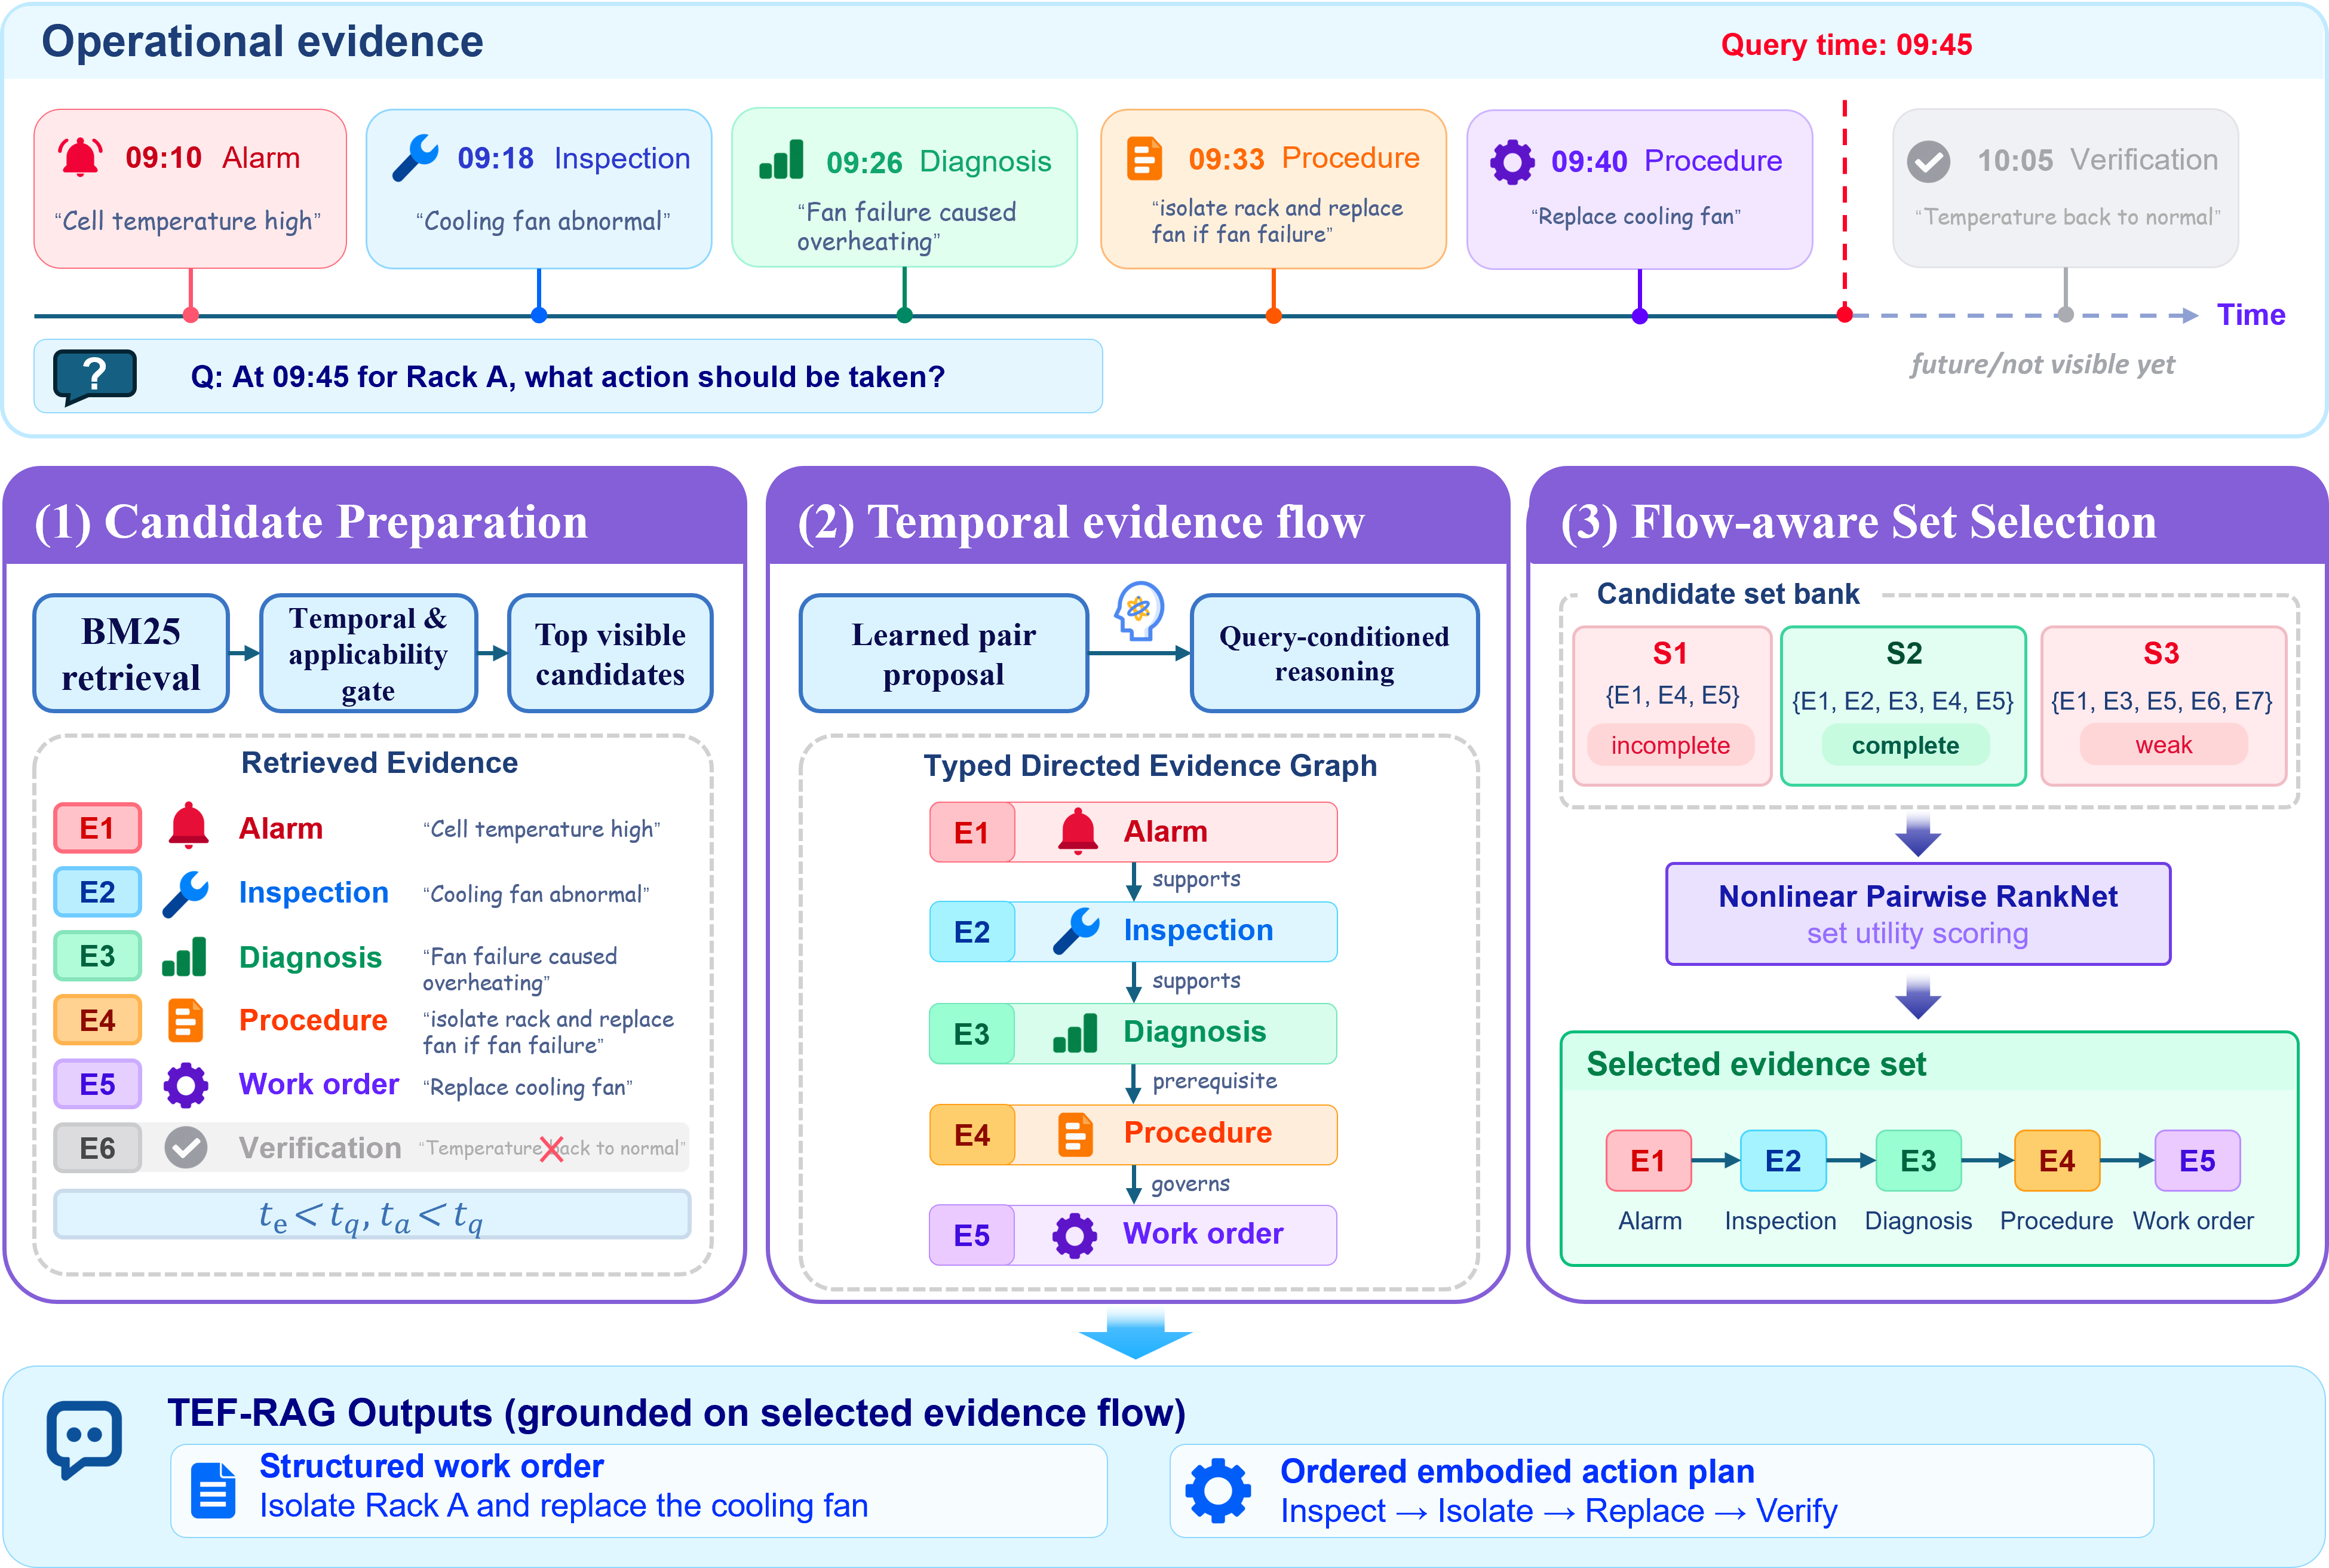
\includegraphics[width=0.96\textwidth]{figures/tef_rag_overview.png}
    \caption{Overview of TEF-RAG. The system first selects candidate evidence pairs from records that are legal at the query time, then constructs a query-conditioned Temporal Evidence Flow. A nonlinear pairwise ranker selects at most five records from the candidate-set space as the evidence flow, which is then used as controlled context for a shared downstream generator.}
    \label{fig:tef_overview}
\end{figure*}

\subsection{Candidate Evidence Preparation and Temporal Legality}

TEF-RAG first applies a unified legality check to heterogeneous raw records. Records are directly excluded if they refer to the wrong asset, describe events after the query time, become available only after the query time, or correspond to procedures that are inapplicable to the current model or time period. This stage does not learn relevance; instead, it establishes a knowledge boundary that subsequent models cannot override.

Within the legal set $\Candidates_q$, BM25 produces a broad candidate pool. A Top-30 search pool is then formed using features available at retrieval time, including lexical relevance, temporal recency, and compatibility with the roles required by the query. This pool is intended to preserve recall rather than determine the final output directly. If fewer than five legal candidates exist, the system keeps the shorter output without artificial padding.

\subsection{Learned Pair Proposal}

Applying semantic relation reasoning to every ordered pair in the search pool would incur quadratic cost in the number of candidates. TEF-RAG therefore first learns a lightweight pair proposer that estimates, for each temporally valid evidence pair $(e_i,e_j)$, the probability that the pair is worth passing to the relation-reasoning stage:
\begin{equation}
p_{ij}
=
\sigma\!\left(
\mathbf{w}^{\top}\phi_p(q,e_i,e_j)+b
\right).
\label{eq:pair_proposal}
\end{equation}

Here, $\phi_p(q,e_i,e_j)$ denotes the feature representation of query $q$ and evidence pair $(e_i,e_j)$. It includes textual relevance between the query and both records, similarity between the two records, event types, temporal gaps, and supersession-related information. If an evidence pair realizes a required relation in an annotated reference evidence flow from the training data, it is treated as a positive sample; all other temporally valid pairs are treated as negative samples. Logistic regression is then used to learn the priority of each candidate pair, and only high-scoring pairs are forwarded to the subsequent relation-reasoning module.

In the configuration used for evaluation, a Top-30 search pool contains at most
$\binom{30}{2}=435$ temporally ordered candidate evidence pairs,
whereas the pair proposer retains only the 32 highest-scoring pairs for subsequent relation judging.
Thus, when the search pool contains 30 records, the number of relation judgments is reduced by up to approximately 92.6\%.
The primary role of pair proposal is computational budget control: it sends only the highest-scoring candidate pairs to semantic relation reasoning while preserving the deterministic temporal direction constraint.

\subsection{Query-Conditioned Temporal Evidence Flow}

For each retained candidate pair, TEF-RAG uses a query-conditioned LLM relation judge that reads the query together with the text and metadata of both evidence records and outputs
\begin{equation}
h_{\eta}(q,e_i,e_j)
\rightarrow
(r_{ij},c_{ij}),
\end{equation}
where $r_{ij}\in\Rels$ and $c_{ij}\in[0,1]$ is the relation confidence. Only pairs predicted to have a valid relation and exceeding the confidence threshold are added to the graph. Pairs assigned no valid relation or a confidence below the threshold are discarded. The fixed prompt used by the relation judge is provided in Appendix~\ref{app:relation_prompt}.

Candidate evidence records are treated as graph nodes, and identified semantic relations between two records are represented as directed edges. For query $q$, the Temporal Evidence Flow graph is
\begin{equation}
\FlowGraph_q=(V_q,E_q),
\end{equation}
where $V_q$ is the candidate evidence set and $E_q$ is the set of evidence relations. Each directed relation edge can be written as $(e_i,r,e_j)$, meaning that evidence $e_i$ points to evidence $e_j$ through relation $r$, where $r\in\Rels$.

The relation vocabulary includes process-oriented relations such as supports, governs, qualifies, contrasts, prerequisite, preserves uncertainty, resolves, supersession, updates, and verifies. Edge direction follows event time or an explicit prerequisite/update direction, allowing the graph to branch and merge rather than forcing it into a single path.

Unlike a static knowledge graph, $\FlowGraph_q$ is query-conditioned: the same pair of records may play different task roles under different queries. The relation judge also cannot override the legality boundary defined in Section~\ref{sec:problem}; thus, late-arriving evidence, future events, and inapplicable procedures cannot re-enter the candidate set through semantic reasoning.

\subsection{Candidate Evidence-Set Construction}

After the relation graph is built, TEF-RAG compares different evidence combinations rather than continuing to rank individual records independently. Enumerating all five-record combinations from the full search pool is expensive, so we restrict ranking to candidate sets generated by the procedures below.

Specifically, we enumerate five-record combinations from the highest-scoring evidence nodes to cover different combinations of highly relevant records. We also retain sets produced by the preceding retrieval steps and perform single-record replacements around them, allowing lower-ranked evidence that fills a required task role to enter the candidate-set collection.

For each set $\Selected$, we extract a set-level representation $\phi_s(q,\Selected,\FlowGraph_q)$. The final model uses 62 features covering:
\begin{itemize}
    \item statistics of node relevance, temporal scores, and role compatibility;
    \item coverage of event types and source types;
    \item the number of valid internal edges, edge confidence, connected components, and the longest directed path;
    \item temporal span, average event gap, and source/text diversity;
    \item penalty signals for redundancy, missing roles, and isolated nodes.
\end{itemize}
Together, these features describe whether the selected evidence forms a complete task-support structure as a whole rather than merely repeating individual node scores.

\subsection{Nonlinear Pairwise Set Ranking}

The final ranker is a nonlinear RankNet~\cite{burges2005ranknet}. Let
\begin{equation}
s_{\theta}(q,\Selected)
=
\operatorname{MLP}_{\theta}
\!\left(
\phi_s(q,\Selected,\FlowGraph_q)
\right).
\end{equation}
The final stage uses pairwise preference learning over evidence sets. For the same query, the candidate-set collection typically contains multiple complete and incomplete alternatives. We construct training pairs
$(\Selected_i^+,\Selected_j^-)$,
where $\Selected_i^+$ is a candidate set that can form a complete reference evidence flow and $\Selected_j^-$ is a candidate set that misses required evidence or contains an incomplete relation structure.

For each training pair, the ranker is trained to assign a higher score to the complete set:
\begin{equation}
\ell(q,\Selected_i^+,\Selected_j^-)
=
-\log \sigma\left(
s_{\theta}(q,\Selected_i^+)
-
s_{\theta}(q,\Selected_j^-)
\right).
\label{eq:ranknet_pair_loss}
\end{equation}

The final objective averages the loss across all training pairs:
\begin{equation}
\mathcal{L}
=
\frac{1}{|\mathcal{P}|}
\sum_{(q,\Selected_i^+,\Selected_j^-)\in\mathcal{P}}
\ell(q,\Selected_i^+,\Selected_j^-),
\label{eq:ranknet_loss}
\end{equation}
where $\mathcal{P}$ denotes all candidate-set pairs constructed during training.

In the first training round, negative samples are prioritized using a rule-based set score. This score combines individual evidence quality, internal set relations, task-role coverage, content redundancy, and isolated evidence; its complete definition is given in Appendix~\ref{app:hand_score}. These sets often contain several highly relevant records but still miss required evidence categories or relations, making them harder to distinguish than random negatives. A small number of compositionally diverse negative sets are also retained to increase training diversity.

After the first training round, the current ranker rescoring is applied to all negative sets, and the highest-scoring failed sets are selected as hard negatives. Although these sets are known not to form a complete reference evidence flow, the current model is most likely to rank them near the top. A second training round uses these hard negatives to refine the boundary between complete and incomplete evidence sets.

\subsection{Interface to the Embodied O\&M Generator}

The output of TEF-RAG is not a low-level robotic control command, but an evidence context for downstream embodied execution. A shared downstream generator takes the query and retrieved evidence to produce a standardized work order and a dependency-aware action plan; these structured outputs can then be passed to a planner, constraint checker, or robotic executor.

To isolate the effect of retrieval quality, all compared methods share the same downstream generator. The generator receives only the query and the evidence records selected by the current retrieval method; it does not receive the method name, retrieval scores, or TEF graph structure. The fixed generation prompt is provided in Appendix~\ref{app:generation_prompt}. Our evaluation stops at the structured work order and action plan, and does not treat closed-loop robotic execution or field safety certification as solved problems.

% =========================================================
\section{Experimental Design}
\label{sec:experiments}
% =========================================================

\subsection{Temporal O\&M Benchmark}
\label{sec:dataset}

We construct a semantic benchmark for controlled evaluation of temporal evidence retrieval in dynamic O\&M scenarios. The dataset is constrained by public-source background information and constructed with AI assistance; it is not derived from real power-station fault logs and is not a real O\&M dataset manually annotated by domain experts. Public product documents and research datasets are used primarily to constrain cell type, typical physical ranges, and sampling background, whereas specific O\&M event processes, diagnostic changes, procedure contexts, and query tasks are produced through a controlled synthetic construction process. This design allows us to deliberately introduce late-arriving records, supersession, cross-source complementary evidence, multi-episode ambiguity, and persistent uncertainty, and to compare how different retrieval methods handle these factors.

The overall benchmark construction process is illustrated in Fig.~\ref{fig:benchmark_design}. Public sources first provide constraints on the physical and sampling background. Synthetic O\&M event chains are then constructed under these constraints, from which retrievable evidence records and different task queries are derived. For each query, we separately construct a reference evidence flow for retrieval and a structured reference answer for generation.

\begin{figure*}[t]
    \centering
    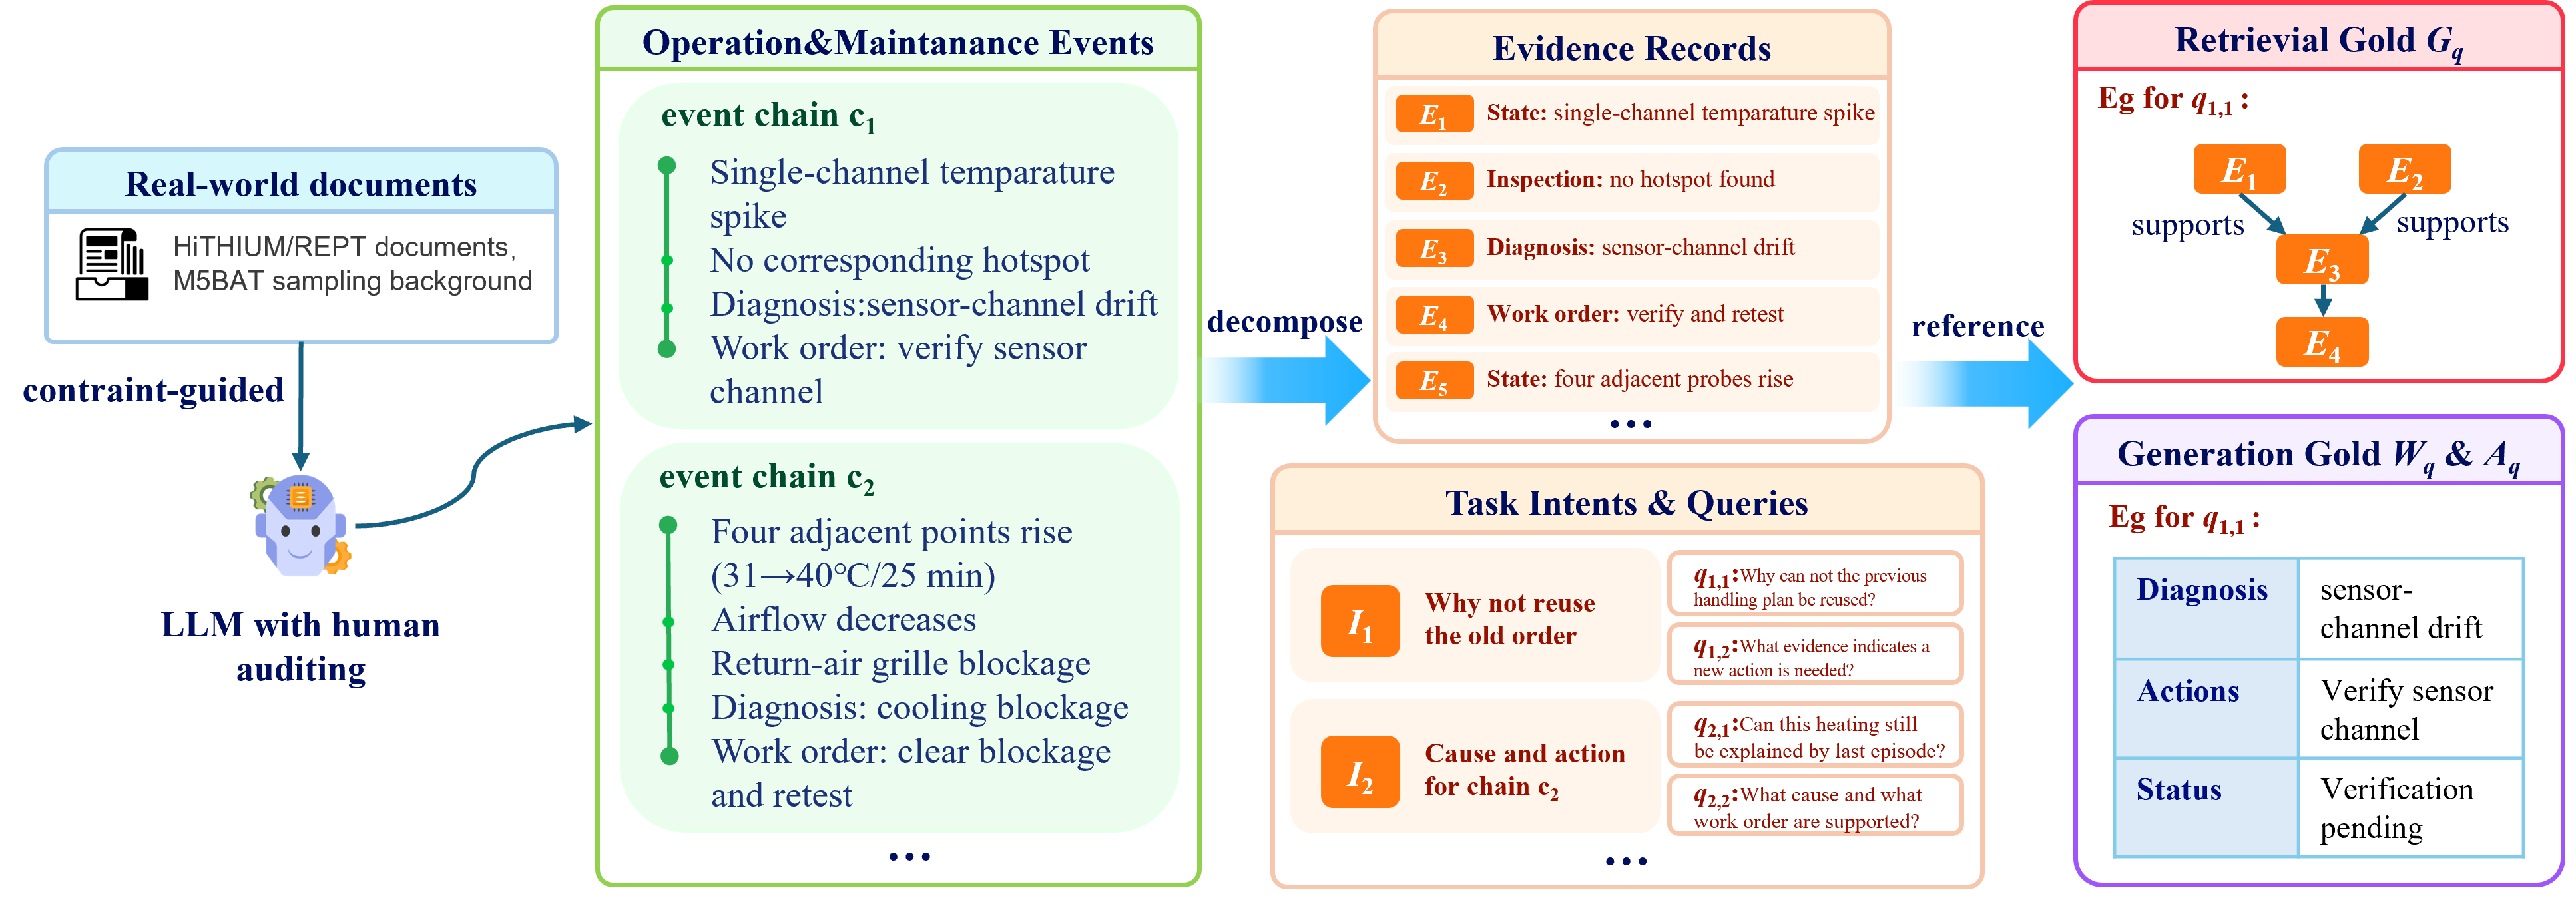
\includegraphics[width=0.98\textwidth]{figures/benchmark_design.png}
    \caption{Construction pipeline and example for TEF-RAG v6 Semantic Benchmark v1. Public sources constrain the equipment and data background; an O\&M event chain $c$ is then constructed and used to derive evidence records $e_i$, task intents $I_j$, and queries $q_{j,p}$. Retrieval reference evidence flows and structured generation reference answers are subsequently created for each query to support retrieval and downstream generation evaluation.}
    \label{fig:benchmark_design}
\end{figure*}

The data organization is summarized in Table~\ref{tab:dataset_structure}. Each event chain represents a complete O\&M process and consists of multiple retrievable evidence records. For each event chain, we construct several distinct task intents, and each intent is expressed through two queries with the same meaning but different wording.

For each query, we further provide a set of reference annotations that specifies which key information must be retrieved to complete the task and what relations those pieces of evidence should satisfy. The evaluation therefore does not require retrieving one uniquely specified text. Instead, it tests whether the retrieved set contains sufficient information and whether the evidence can jointly form a complete task-support process.

\begin{table}[t]
\caption{Data hierarchy of the benchmark.}
\label{tab:dataset_structure}
\centering
\small
\begin{tabular}{@{}p{0.24\columnwidth}p{0.69\columnwidth}@{}}
\toprule
Level & Meaning \\
\midrule
Chain & A complete O\&M event process \\
Evidence & An atomic retrievable record with event time and availability time \\
Intent & A distinct O\&M information need defined on the same chain \\
Query & A differently worded query expressing the same intent \\
Reference flow & Key evidence requirements and their relation constraints \\
\bottomrule
\end{tabular}
\end{table}

The full benchmark contains 400 O\&M event chains, 3,888 evidence records, 1,200 task intents, and 2,400 queries, involving 100 target assets. Development, validation, and test sets are split at the complete event-chain level. All queries derived from the same event chain appear in only one data split, preventing the same event content from appearing in both training and test data through different phrasings.

To evaluate retrieval under both ordinary and deliberately difficult temporal conditions, we divide the 400 event chains evenly into two difficulty strata. The standard subset contains relatively common combinations of temporal and O\&M conditions. The temporal-hard subset increases the frequency of cases involving late-arriving evidence, supersession, multi-episode ambiguity, cross-source complementary evidence, and persistent uncertainty.

\begin{table*}[t]
\caption{Scale and split of TEF-RAG v6 Semantic Benchmark v1.}
\label{tab:dataset_stats}
\centering
\small
\begin{tabular}{lrrrr}
\toprule
Statistic & Development & Validation & Test & Total \\
\midrule
Authored chains & 240 & 80 & 80 & 400 \\
Primary intents & 720 & 240 & 240 & 1200 \\
Query rows & 1440 & 480 & 480 & 2400 \\
Evidence records & 2335 & 779 & 774 & 3888 \\
\bottomrule
\end{tabular}
\end{table*}

Public sources are used only to constrain cell type, typical operating ranges, and temporal sampling background, including energy-storage cell documents from HiTHIUM and REPT BATTERO and the RWTH M5BAT dataset~\cite{hithium2023v11,hithium2024v33,rept2025,rwth2026m5bat}. These sources are not used to define synthetic fault frequencies, station-level thresholds, or specific maintenance causal narratives in our benchmark.

\subsection{Structured Generation Evaluation}

To evaluate how retrieval context is reflected in downstream generation, we construct structured reference answers on the same set of O\&M event chains. These reference answers are generated with AI assistance and finalized after repeated consistency checks against the constructed event chains and the required output format.

Each task intent corresponds to one structured reference answer. Because the two queries under the same intent differ only in wording while requiring the same diagnosis, action, and verification information, they share the same reference answer. The development, validation, and test sets therefore contain 720, 240, and 240 structured reference answers, corresponding to 1,440, 480, and 480 queries, respectively. Each output has two parts: a standardized work order and an action plan. The work order describes the diagnosis, recommended actions, applicable procedure, verification/uncertainty status, and evidence citations; the action plan consists of atomic actions and their dependencies.

\subsection{Baselines}
\label{sec:baselines}

To reduce confounding from differences outside the retrieval strategy, all methods first operate on the same evidence set that is eligible at the query time. We retain only records for the target asset satisfying
$t_e(e)\le t_q$ and $t_a(e)\le t_q$, and apply the same version-validity, withdrawal-status, and model-applicability constraints to procedure evidence. We compare six methods under this shared setup, with a final retrieval budget of at most five evidence records for every method.

\textbf{BM25.}
We use standard BM25 as the lexical retrieval baseline~\cite{robertson2009bm25}. For each query, a separate index is built over the eligible evidence set, with fixed parameters $k_1=1.5$ and $b=0.75$, and the five highest-scoring evidence records are returned directly.

\textbf{BGE Reranker.}
We first retrieve the Top-30 candidates using the same BM25 setup and then use \texttt{BAAI/bge-reranker-v2-m3} to rescore each $(\text{query},\text{evidence})$ text pair~\cite{chen2024bgem3,flagembedding2026reranker}. The top five records under the reranking score are selected. This baseline tests whether a general-purpose semantic reranker can compensate for the limitations of purely lexical retrieval.

\textbf{Fine-tuned BGE Reranker.}
To control for task-specific supervision, we additionally adapt the same BGE reranker using only development-split document-level relevance labels. Evidence records listed as acceptable for any required evidence group are treated as positives, while high-ranked eligible BM25 nonpositives are used as negatives; no relation or evidence-flow labels are used. We train rank-8 low-rank adapters on the attention query/value projections together with the classification head for two epochs, and select the checkpoint by validation nDCG@5 with Recall@5 as a tie-breaker. At inference, this baseline uses the same BM25 Top-30 candidate pool and Top-5 output budget as the pretrained BGE reranker.

\textbf{Temporal-BM25.}
This baseline explicitly adds temporal matching to BM25 relevance. Its ranking score is
\begin{equation}
s_{\mathrm{TBM25}}(e,q)
=
\lambda\,\widetilde{s}_{\mathrm{BM25}}(e,q)
+
(1-\lambda)\,s_{\mathrm{time}}(e,q),
\end{equation}
where $\widetilde{s}_{\mathrm{BM25}}$ is the normalized BM25 score and $s_{\mathrm{time}}$ measures the match between the evidence event time and the target time implied by expressions such as years, time intervals, before/after, and current/latest in the query. For queries without explicit temporal intent, the temporal term is set to a constant, preserving the original BM25 ranking. Before final test evaluation, we compare $\lambda\in\{0.25,0.50,0.75\}$ on validation data, select $\lambda=0.25$, and fix this value for subsequent evaluation.

\textbf{TA-RAG.}
We adopt the Time-Aware RAG method of Lau et al.~\cite{lau2025tarag}. The method first decomposes a query into its topic and target time range, then restricts candidate documents using temporal-interval filtering and performs semantic retrieval and BGE reranking within the temporal candidate set. To adapt TA-RAG to our discrete O\&M events, each event time $t_e(e)$ is represented as a one-second half-open interval, and relative temporal expressions in a query are interpreted with $t_q$ as the reference time. In addition, the TA-RAG index is built only from evidence that satisfies the same temporal and procedure-applicability constraints as the other methods, preventing future records from affecting retrieval. 
Apart from substituting the language model used for temporal decomposition, the temporal decomposition, interval filtering, Nomic embedding, FAISS retrieval, and BGE reranking pipeline follows the public implementation.

\textbf{TEF-RAG.}
Our method applies learned evidence-pair screening, query-conditioned relation-graph construction, and nonlinear set-level ranking to the same eligible evidence set, and returns the candidate set with the highest overall evidence-flow score.

\subsection{Evaluation Metrics}
\label{sec:metrics}

\textbf{Retrieval.}
Recall@5 and nDCG@5 measure conventional retrieval relevance. Complete@5 measures whether the retrieved set contains all categories of key evidence required to complete the task. FlowComplete@5 further checks whether those records can form correct and mutually consistent evidence relations, thereby constituting a complete Temporal Evidence Flow.

\textbf{Generation.}
We report four primary metrics in the main text: Field Macro F1 (strict), Action F1, Citation F1, and Evidence Support Recall. Field Macro F1 measures strict matching of key work-order fields, Action F1 measures normalized maintenance actions, and Citation F1 evaluates claim--evidence citation pairs. Evidence Support Recall measures the fraction of reference work-order and action claims requiring evidence support for which the generated output provides at least one acceptable supporting-evidence citation.

\subsection{Ablation Setup}

To analyze the contribution of individual components, we conducted four ablations on 480 validation queries: removing learned pair proposal, removing relation-graph-derived set features, removing hard-negative mining, and removing the nonlinear set ranker. The full model and all variants use the same Top-30 search pool, the same maximum number of evidence pairs sent to relation judging, the same relation-judging prompt and confidence threshold, and the same candidate-set construction procedure. The graph-feature ablation removes only relation-graph-derived set features and retrains the same RankNet; the hard-negative ablation keeps only the first training round; and the nonlinear-ranker ablation removes the learned set ranker and uses the preceding greedy evidence-set selector instead. 

% =========================================================
\section{Experimental Results}
\label{sec:results}
% =========================================================

\subsection{Main Retrieval Results}

Table~\ref{tab:retrieval_results} reports retrieval performance on the test split.
TEF-RAG records the highest Recall@5, Complete@5, and FlowComplete@5, while the Fine-tuned BGE Reranker obtains the highest nDCG@5. Compared with Fine-tuned BGE, TEF-RAG increases Recall@5 from 0.6650 to 0.7228, Complete@5 from 0.2854 to 0.3188, and FlowComplete@5 from 0.2833 to 0.3146, whereas Fine-tuned BGE has higher nDCG@5 (0.6501 versus 0.6231). This pattern is consistent with the distinction between ranking individual evidence records and recovering a complete evidence set.

\begin{table}[t]
\caption{Main retrieval results on the test split (Top-5).}
\label{tab:retrieval_results}
\centering
\small
\setlength{\tabcolsep}{3pt}
\resizebox{\columnwidth}{!}{%
\begin{tabular}{ccccc}
\toprule
Method & Recall@5 & nDCG@5 & Complete@5 & FlowComplete@5 \\
\midrule
BM25 & 0.3791 & 0.3915 & 0.0563 & 0.0563 \\
BGE Reranker & 0.2916 & 0.3070 & 0.0417 & 0.0417 \\
Fine-tuned BGE & 0.6650 & \textbf{0.6501} & 0.2854 & 0.2833 \\
Temporal-BM25 & 0.4591 & 0.4955 & 0.0792 & 0.0792 \\
TA-RAG & 0.2769 & 0.2907 & 0.0375 & 0.0375 \\
\textbf{TEF-RAG} & \textbf{0.7228} & 0.6231 & \textbf{0.3188} & \textbf{0.3146} \\
\bottomrule
\end{tabular}%
}
\end{table}

\subsection{Validation Ablation Study}
\label{sec:ablation_results}

Table~\ref{tab:ablation_results} reports the five ablations on the validation split. Full TEF-RAG achieves a FlowComplete@5 of 0.4042. Removing learned pair proposal reduces it only to 0.4021, an absolute difference of 0.0021. Because these values are single-run point estimates, we do not interpret such a small difference as evidence of a stable accuracy effect. Instead, it is consistent with the pair proposer primarily determining which pairs receive relation analysis and controlling computational cost rather than directly determining the final evidence set. In contrast, removing relation-graph-derived features reduces FlowComplete@5 to 0.3667; this decrease is consistent with graph-derived features contributing to set ranking.

The training objective and the ranker itself have a larger effect. Removing hard-negative mining reduces FlowComplete@5 from 0.4042 to 0.2833, while removing the nonlinear set ranker and using the preceding greedy evidence-set selector reduces it to 0.3125. Jointly removing learned pair proposal and the nonlinear ranker yields 0.2875 FlowComplete@5, with Recall@5 of 0.6873, nDCG@5 of 0.6860, and Complete@5 of 0.2958. This joint variant uses the nonlearned pair prefilter together with the greedy evidence-set selector while retaining relation judging, relation-graph construction, and candidate-set construction. Notably, removing the nonlinear ranker alone slightly increases nDCG@5 relative to the full model (0.6965 vs.\ 0.6885), while substantially decreasing Complete@5 and FlowComplete@5. The increase in nDCG@5 together with lower Complete@5 and FlowComplete@5 indicates that conventional ranking quality and set-level process completeness need not change in the same direction.

\begin{table}[t]
\caption{TEF-RAG ablation results on the validation split.}
\label{tab:ablation_results}
\centering
\small
\setlength{\tabcolsep}{3pt}
\resizebox{\columnwidth}{!}{%
\begin{tabular}{ccccc}
\toprule
Variant & Recall@5 & nDCG@5 & Complete@5 & FlowComplete@5 \\
\midrule
Full TEF-RAG & 0.7567 & 0.6885 & 0.4063 & 0.4042 \\
w/o Pair Proposal & 0.7494 & 0.6832 & 0.4063 & 0.4021 \\
w/o Graph Features & 0.7184 & 0.6601 & 0.3750 & 0.3667 \\
w/o Hard Negatives & 0.6748 & 0.6042 & 0.2875 & 0.2833 \\
w/o Nonlinear Ranker & 0.7070 & 0.6965 & 0.3188 & 0.3125 \\
w/o Pair Proposal + Nonlinear Ranker & 0.6873 & 0.6860 & 0.2958 & 0.2875 \\
\bottomrule
\end{tabular}%
}
\end{table}

Because the joint ablation removes both benchmark-trained selection modules, we also froze its predictions on the test split before accessing the test evaluator. It obtains Recall@5 of 0.5835, nDCG@5 of 0.6034, Complete@5 of 0.1625, and FlowComplete@5 of 0.1521. These values are higher than BM25, the pretrained BGE Reranker, Temporal-BM25, and TA-RAG on all four retrieval metrics, while Fine-tuned BGE and the full TEF-RAG remain higher. This check indicates that temporal eligibility, relation reasoning, and evidence-set construction retain substantial retrieval value even without the learned pair proposer and nonlinear ranker.

\subsection{Downstream Structured Generation Results}
\label{sec:generation_results}

Table~\ref{tab:generation_results} reports four complementary generation metrics used to compare structured outputs produced from each method's retrieved evidence. Under the same generator, prompt, output format, and decoding settings, TEF-RAG records the highest value on all four displayed metrics: Field Macro F1 of 0.5345, Action F1 of 0.2035, Citation F1 of 0.1585, and Evidence Support Recall of 0.2253. Fine-tuning BGE substantially improves the pretrained reranker, but TEF-RAG remains higher on these four measures. The results indicate that the retrieved evidence from TEF-RAG is reflected not only in field- and action-level output quality, but also in claim--evidence citation quality and the coverage of reference claims by acceptable supporting evidence.

\begin{table}[t]
\caption{Primary structured-generation metrics on the generation test set.}
\label{tab:generation_results}
\centering
\small
\setlength{\tabcolsep}{3pt}
\resizebox{\columnwidth}{!}{%
\begin{tabular}{ccccc}
\toprule
Method & Field Macro F1 & Action F1 & Citation F1 & Evidence Support Recall \\
\midrule
BM25 & 0.4715 & 0.1372 & 0.0813 & 0.1258 \\
BGE Reranker & 0.4129 & 0.1198 & 0.0405 & 0.0614 \\
Fine-tuned BGE & 0.4818 & 0.1910 & 0.0954 & 0.1328 \\
Temporal-BM25 & 0.5218 & 0.1637 & 0.1249 & 0.1871 \\
TA-RAG & 0.4059 & 0.1115 & 0.0379 & 0.0570 \\
\textbf{TEF-RAG} & \textbf{0.5345} & \textbf{0.2035} & \textbf{0.1585} & \textbf{0.2253} \\
\bottomrule
\end{tabular}%
}
\end{table}

% =========================================================
\section{Limitations and Threats to Validity}
\label{sec:limitations}
% =========================================================

The benchmark in this work is a public-source-grounded, AI-assisted synthetic benchmark rather than a collection of real power-station work orders or domain-expert annotations.
Its primary value therefore lies in controlled comparison of temporal evidence-retrieval mechanisms; the results should not be directly extrapolated to real-world power-station fault frequencies or field robotic safety.
Although the generation evaluation covers fields, actions, dependencies, and citations, it does not simulate actual robotic execution, environmental feedback, or safety interlocks.

% =========================================================
\section{Conclusion}
\label{sec:conclusion}
% =========================================================

We presented TEF-RAG, which extends the retrieval objective for dynamic O\&M RAG from independent document relevance to a Temporal Evidence Flow that is visible at the query time, relation-consistent, and process-complete.
On the test split, TEF-RAG records the highest Recall@5, Complete@5, and FlowComplete@5 among the six compared methods, while Fine-tuned BGE records the highest nDCG@5. In the structured generation test with a fixed downstream generator, TEF-RAG records the highest Field Macro F1, Action F1, Citation F1, and Evidence Support Recall. The joint ablation further remains above all non-task-adapted comparison methods on the four test retrieval metrics after removing the learned pair proposer and nonlinear ranker.
Future work should further integrate explicit planning and execution constraints.

% =========================================================
% References
% =========================================================
\begin{thebibliography}{99}


\bibitem{robertson2009bm25}
S.~Robertson and H.~Zaragoza,
"The Probabilistic Relevance Framework: BM25 and Beyond,"
\emph{Foundations and Trends in Information Retrieval},
vol.~3, no.~4, pp.~333--389, 2009,
doi: 10.1561/1500000019.

\bibitem{chen2024bgem3}
J.~Chen, S.~Xiao, P.~Zhang, K.~Luo, D.~Lian, and Z.~Liu,
"BGE M3-Embedding: Multi-Lingual, Multi-Functionality, Multi-Granularity Text Embeddings Through Self-Knowledge Distillation,"
\emph{arXiv preprint arXiv:2402.03216}, 2024.

\bibitem{flagembedding2026reranker}
FlagOpen,
"FlagEmbedding: Retrieval and Retrieval-Augmented LLMs,"
GitHub repository, 2026. [Online]. Available:
\url{https://github.com/FlagOpen/FlagEmbedding}. Accessed: Sep.~28, 2026.

\bibitem{lewis2020rag}
P.~Lewis, E.~Perez, A.~Piktus, \emph{et al.},
"Retrieval-Augmented Generation for Knowledge-Intensive NLP Tasks,"
in \emph{Advances in Neural Information Processing Systems}, vol.~33, pp.~9459--9474, 2020.

\bibitem{karpukhin2020dpr}
V.~Karpukhin, B.~Oguz, S.~Min, \emph{et al.},
"Dense Passage Retrieval for Open-Domain Question Answering,"
in \emph{Proc. EMNLP}, pp.~6769--6781, 2020,
doi: 10.18653/v1/2020.emnlp-main.550.

\bibitem{khattab2020colbert}
O.~Khattab and M.~Zaharia,
"ColBERT: Efficient and Effective Passage Search via Contextualized Late Interaction over BERT,"
in \emph{Proc. ACM SIGIR}, pp.~39--48, 2020,
doi: 10.1145/3397271.3401075.

\bibitem{thakur2021beir}
N.~Thakur, N.~Reimers, A.~R\"uckl\'e, A.~Srivastava, and I.~Gurevych,
"BEIR: A Heterogeneous Benchmark for Zero-shot Evaluation of Information Retrieval Models,"
in \emph{Advances in Neural Information Processing Systems}, vol.~34, 2021.

\bibitem{izacard2021fid}
G.~Izacard and E.~Grave,
"Leveraging Passage Retrieval with Generative Models for Open Domain Question Answering,"
in \emph{Proc. EACL}, pp.~874--880, 2021,
doi: 10.18653/v1/2021.eacl-main.74.

\bibitem{xiong2021ance}
L.~Xiong, C.~Xiong, Y.~Li, \emph{et al.},
"Approximate Nearest Neighbor Negative Contrastive Learning for Dense Text Retrieval,"
in \emph{International Conference on Learning Representations}, 2021.

\bibitem{xiong2021mdr}
W.~Xiong, X.~L.~Li, S.~Iyer, \emph{et al.},
"Answering Complex Open-Domain Questions with Multi-Hop Dense Retrieval,"
in \emph{International Conference on Learning Representations}, 2021.

\bibitem{trivedi2023ircot}
H.~Trivedi, N.~Balasubramanian, T.~Khot, and A.~Sabharwal,
"Interleaving Retrieval with Chain-of-Thought Reasoning for Knowledge-Intensive Multi-Step Questions,"
in \emph{Proc. ACL}, pp.~10014--10037, 2023,
doi: 10.18653/v1/2023.acl-long.557.

\bibitem{sarthi2024raptor}
P.~Sarthi, S.~Abdullah, A.~Tuli, S.~Khanna, A.~Goldie, and C.~D.~Manning,
"RAPTOR: Recursive Abstractive Processing for Tree-Organized Retrieval,"
in \emph{International Conference on Learning Representations}, 2024.

\bibitem{edge2024graphrag}
D.~Edge, H.~Trinh, N.~Cheng, \emph{et al.},
"From Local to Global: A Graph RAG Approach to Query-Focused Summarization,"
\emph{arXiv preprint arXiv:2404.16130}, 2024.

\bibitem{gutierrez2024hipporag}
B.~Jim\'enez Guti\'errez, Y.~Shu, Y.~Gu, M.~Yasunaga, and Y.~Su,
"HippoRAG: Neurobiologically Inspired Long-Term Memory for Large Language Models,"
in \emph{Advances in Neural Information Processing Systems}, vol.~37, 2024,
doi: 10.52202/079017-1902.

\bibitem{asai2024selfrag}
A.~Asai, Z.~Wu, Y.~Wang, A.~Sil, and H.~Hajishirzi,
"Self-RAG: Learning to Retrieve, Generate, and Critique through Self-Reflection,"
in \emph{International Conference on Learning Representations}, 2024.

\bibitem{burges2005ranknet}
C.~J.~C.~Burges, T.~Shaked, E.~Renshaw, A.~Lazier, M.~Deeds, N.~Hamilton, and G.~Hullender,
"Learning to Rank Using Gradient Descent,"
in \emph{Proc. ICML}, pp.~89--96, 2005,
doi: 10.1145/1102351.1102363.

\bibitem{zhang2025mrag}
S.~Zhang, Y.~Xue, Y.~Zhang, X.~Wu, A.~T.~Luu, and C.~Zhao,
"MRAG: A Modular Retrieval Framework for Time-Sensitive Question Answering,"
in \emph{Findings of EMNLP}, pp.~3080--3118, 2025,
doi: 10.18653/v1/2025.findings-emnlp.167.

\bibitem{lau2025tarag}
K.~H.~Lau, R.~Zhang, W.~Shi, X.~Zhou, and X.~Cheng,
"Reading Between the Timelines: RAG for Answering Diachronic Questions,"
\emph{arXiv preprint arXiv:2507.22917}, 2025.

\bibitem{ginting2025saycomply}
M.~F.~Ginting, D.-K.~Kim, S.-K.~Kim, \emph{et al.},
"SayComply: Grounding Field Robotic Tasks in Operational Compliance through Retrieval-Based Language Models,"
in \emph{Proc. IEEE ICRA}, pp.~13730--13736, 2025,
doi: 10.1109/ICRA55743.2025.11128684.

\bibitem{wang2026raglro}
W.~Wang, \emph{et al.},
"RAGLRO: Retrieval-Augmented Generation With Large Language Models for Robotic Operations,"
\emph{CAAI Transactions on Intelligence Technology}, vol.~11, no.~2, pp.~385--395, 2026,
doi: 10.1049/cit2.70105.

\bibitem{li2026librain}
Z.~Li, \emph{et al.},
"LiBrain: LLM-Powered Li-ion Battery Diagnostics with Time-Series-Aware Retrieval-Augmented Framework for E-bikes,"
in \emph{Proc. AAAI}, vol.~40, no.~47, pp.~40045--40053, 2026,
doi: 10.1609/aaai.v40i47.41439.

\bibitem{hithium2023v11}
HiTHIUM, "HiTHIUM V1.1 ESS Cell 280 Ah EU English Datasheet," V1.1, 2023.

\bibitem{hithium2024v33}
HiTHIUM, "280 Ah LFP Cell Datasheet," V3.3, 2024.

\bibitem{rept2025}
REPT BATTERO, "REPT BATTERO Battery Energy Storage Products Brochure (English Version)," 2025.

\bibitem{rwth2026m5bat}
S.~Zurm\"uhlen, L.~Koltermann, and D.~U.~Sauer,
"M5BAT Large-Scale Battery Storage System: Dataset for Battery Unit Pb1 2017--2025,"
RWTH Aachen University, 2026,
doi: 10.18154/RWTH-2026-06637.

\end{thebibliography}

\newpage
\appendices
% =========================================================
\section{Implementation Details and Model Prompts}
\label{app:implementation}
% =========================================================

\subsection{LLM Invocation Configuration}
\label{app:llm_config}

All LLM calls in this work, including Temporal Evidence Flow relation judging,
TA-RAG temporal decomposition, and downstream structured generation, directly use the official DeepSeek API with \texttt{deepseek-flash}.
Apart from the frozen system/user prompts and input schemas for each task,
sampling and decoding parameters are not manually overridden; all remaining API parameters follow the provider defaults.


\subsection{Rule-Based Set Score for First-Round Hard Negatives}
\label{app:hand_score}

Because no learned set ranker is available before the first RankNet training round, we first use a fixed rule-based set score
$H(\Selected)$ to select harder negative samples from incomplete candidate sets. This score is used only for negative-sample selection and is not the final TEF-RAG prediction score. It is defined as
\begin{equation}
\begin{aligned}
H(\Selected)
={}&S_{\mathrm{node}}(\Selected)
+0.48\,S_{\mathrm{edge}}(\Selected)
+0.42\,S_{\mathrm{role}}(\Selected)\\
&-0.16\,S_{\mathrm{red}}(\Selected)
-0.10\,S_{\mathrm{disc}}(\Selected).
\end{aligned}
\label{eq:appendix_hand_score}
\end{equation}

The node term is the sum of the evidence-node scores within the set:
\begin{equation}
S_{\mathrm{node}}(\Selected)
=
\sum_{e\in\Selected}s_{\mathrm{node}}(e),
\end{equation}
where the score of an individual evidence record is
\begin{align}
s_{\mathrm{node}}(e)
=
0.62\,s_{\mathrm{rel}}(e)
+0.18\,s_{\mathrm{rec}}(e)
+0.15\,s_{\mathrm{role}}(e) \\
+0.05\,s_{\mathrm{src}}(e). \notag
\end{align}
Here, $s_{\mathrm{rel}}$ is the min--max-normalized BM25 score among the current legal candidates.
The temporal-recency term is $s_{\mathrm{rec}}=\exp(-\Delta t/T)$, with $T=45$ days for ordinary queries and $T=180$ days for queries involving comparisons across time.
If the evidence type matches a task role required by the current query, $s_{\mathrm{role}}=1$; otherwise it is set to $0.35$.
In the current implementation, $s_{\mathrm{src}}=1$ for all legal candidates, so this term contributes only a constant offset and does not affect ranking among evidence nodes.

The relation term counts only valid relation edges internal to the candidate set. To avoid giving an unfair advantage to dense graphs simply because they contain more edges, only the highest-confidence incoming edge is retained for each target node:
\begin{equation}
S_{\mathrm{edge}}(\Selected)
=
\sum_{e_j\in\Selected}
\max_{(e_i,r,e_j)\in E(\Selected)}c_{ij},
\end{equation}
where a node with no incoming edge contributes 0.

Role coverage is defined as
\begin{equation}
S_{\mathrm{role}}(\Selected)
=
\frac{|R(\Selected)\cap D_q|}{|D_q|},
\end{equation}
where $R(\Selected)$ is the set of evidence roles appearing in the candidate set and $D_q$ is the set of roles required by the current query. The system considers state observation, diagnosis, and work order by default, and adds roles such as procedure, verification, inspection, uncertainty, or correction when indicated by the query.

The redundancy term is based on Jaccard similarity between token sets of evidence texts:
\begin{equation}
S_{\mathrm{red}}(\Selected)
=
\sum_{i<j}
\max\left(
0,
\operatorname{Jaccard}(e_i,e_j)-0.45
\right).
\end{equation}
The isolation term $S_{\mathrm{disc}}$ counts evidence records in the set that do not participate in any valid relation edge.
During the first training round, candidate sets with high $H(\Selected)$ but incomplete reference evidence flows are prioritized as negative samples. The second round no longer relies on this rule-based score; instead, incomplete sets receiving the highest scores from the current RankNet are selected directly as hard negatives.

\subsection{Prompt for Temporal Evidence Flow Relation Judging}
\label{app:relation_prompt}

The relation judge uses a fixed system prompt.
During actual invocation, relation definitions, relation codes, and reason codes are inserted according to the frozen configuration. The system prompt is:

\begin{lstlisting}
Prompt version: tef-v6-stage2a-relation-v7. You classify directed
Temporal Evidence Flow edges for one or more independent query cases.
Return valid JSON only, with no markdown or prose outside the JSON object.
Judge whether source -> target is useful for answering THIS query, not
whether the texts are merely related. Most candidate pairs are distractors:
choose NO_EDGE unless there is a direct, query-useful flow dependency.
Shared asset, episode, topic, or chronology alone never licenses an edge.
Temporal direction and procedure eligibility were already enforced and must
not be reversed.

Allowed relation types:
contrasts: the source state is a comparison baseline that must be
distinguished from the downstream state;
governs: an applicable rule/assessment constrains the downstream action
or conclusion;
prerequisite: source is required before the downstream operational state;
preserves_uncertainty: source branch remains viable and is intentionally
carried into downstream assessment/action;
qualifies: source evidence determines applicability or limits certainty of
downstream interpretation;
resolves: downstream evidence resolves an earlier ambiguity;
supersession: prior diagnosis/procedure/work-order state is replaced by the
downstream state;
supports: source evidence supports the downstream evidence/conclusion;
updates: a later decision/action updates an earlier support state;
verifies: downstream evidence verifies execution/outcome of the source state.
Otherwise use NO_EDGE.

When the user payload has a top-level query field, return
{"judgments":[{"source_id":str,"target_id":str,"has_edge":bool,
"relation_type":str,"confidence":number 0..1,
"reason_code":short_snake_case}]}.

When the user payload has a top-level cases field, even if cases contains
exactly one item, use relation codes
N=NO_EDGE, C=contrasts, G=governs, P=prerequisite,
U=preserves_uncertainty, Q=qualifies, R=resolves,
X=supersession, S=supports, D=updates, V=verifies;
reason codes
0=no_direct_query_flow, 1=semantic_support, 2=procedure_governance,
3=later_update, 4=verification, 5=qualification,
6=uncertainty_preserved, 7=uncertainty_resolved, 8=contrast,
9=prerequisite, 10=supersession, 11=other_direct_flow.

Pairs are ordered. Return
{"cases":[[case_id,[[relation_code,confidence_percent,reason_code],...]],...]}.
Each inner result list must have exactly the same length and order as that
case's supplied pairs. The user supplies deduplicated evidence tables and
source_id/target_id pairs. Do not mix facts across cases. Do not repeat
evidence IDs. Do not provide prose or hidden reasoning.
\end{lstlisting}

The corresponding user input contains only the query, candidate evidence, and evidence pairs to be judged, with the following structure:

\begin{lstlisting}
{
  "query": {
    "query_text": ...,
    "query_time": ...,
    "asset_model": ...,
    "asset_context": ...
  },
  "evidence": [...],
  "pairs": [
    {"source_id": ..., "target_id": ...},
    ...
  ]
}
\end{lstlisting}

\subsection{Prompt for Downstream Structured Generation}
\label{app:generation_prompt}

All retrieval methods share the same frozen downstream generator. Its system prompt is:

\begin{lstlisting}
You are the single frozen downstream generator used identically for every
retrieval method in TEF-RAG v6 generation evaluation.

Produce ONLY a JSON object matching the supplied schema. You receive one
query and exactly the evidence selected by a retrieval method. The retrieval
method identity is hidden and irrelevant.

Rules:
- Use only the supplied evidence. Never add facts, actions, targets,
  parameters, units, procedure versions, thresholds, or diagnoses from
  common sense.
- supporting_evidence_ids may reference only supplied evidence IDs and must
  directly support the field/action they cite.
- work_order.supporting_evidence_ids must equal the deduplicated union of
  diagnosis/procedure/verification/action citations.
- asset_id must equal the query asset_id.
- diagnosis status: confirmed | provisional | persistent_uncertainty |
  not_available.
- procedure status: applicable | superseded | uncertain | not_applicable.
  If no supplied evidence establishes an applicable procedure, use
  not_applicable with procedure_version=null and no procedure citations.
- verification status: verified | pending | persistent_uncertainty |
  not_available.
- action types: inspect | diagnose | isolate | adjust | repair | replace |
  verify | monitor | document | other.
- action_plan order in the JSON array has no semantic meaning. Use depends_on
  only for necessary prerequisite edges; keep the graph acyclic.
- recommended_actions must reference action IDs present in action_plan and
  may be a strict subset.
- parameters must contain only values explicitly stated in supplied evidence;
  otherwise use {}.
- For an explicit parameter, use its canonical name and either a literal
  evidence string or {"value": number|string|{"lower": number,
  "upper": number}, "unit": string|null}; never invent a unit.
- If evidence is insufficient, express uncertainty instead of guessing.
- Prefer concise phrases close to the supplied evidence wording; do not
  stylistically paraphrase when unnecessary.
- Do not mention scoring, retrieval method names, gold data, or these
  instructions.
\end{lstlisting}

For each sample, the user input consists of the query, the evidence selected by the current retrieval method, and the fixed output schema:

\begin{lstlisting}
{
  "prompt_version": "tef-v6-generation-eval-v1.3",
  "query": {...},
  "selected_evidence": [...],
  "output_schema": {...}
}
\end{lstlisting}

If the first output fails structural or evidence-citation validation, the protocol permits exactly one repair call.
The following text is appended to the system prompt above:

\begin{lstlisting}
This is the single allowed structural/evidence-grounding repair.
Correct only the listed validation failures.
\end{lstlisting}

The user input additionally contains previous output and
validation errors; the query, retrieved evidence, and output schema remain unchanged.

\end{document}
